\documentclass{article}
%Seitenränder
\usepackage{geometry}
\geometry{a4paper, left=30mm, right=30mm, top=25mm, bottom=25mm} 

%Encoding:
\usepackage{t1enc}
\usepackage[utf8]{inputenc}

%Mathematische Formeln:
\usepackage{amsmath}
\usepackage{amsfonts}
\usepackage{amssymb}
\usepackage{mathtools} %Erweitert das amsmath package
\usepackage{yhmath} %Erweiterte Schriftarten in Mathe-Umgebungen

\usepackage{graphicx}
\usepackage{framed}
% for \Yleft \Yright
\usepackage{stmaryrd}
\usepackage{xcolor} %Text und Grafiken farbig gestalten
\usepackage{multicol} %Mehrspaltiger Text

\usepackage{hyperref} %Verwandelt u.a. interne links in klickbare Verweise
\usepackage{enumitem} %itemize, enumerate, description individuell anpassen
\usepackage{float} %Grafiken schöner einfügen
\usepackage{wrapfig} %Von Text umflossene Grafiken einfügen
\usepackage{tikz} %Automaten, Graphen, ... mit LaTeX darstellen
\usetikzlibrary{arrows,shapes,automata,petri,backgrounds,calc,intersections}

\usepackage{todonotes}
\usepackage[toc]{appendix}


% Titel in Kopfzeilen
\usepackage{fancyhdr}
\pagestyle{fancy}
\setlength{\headheight}{20pt}


% Format der Autorenkürzel definieren
\newcommand{\initials}[1]{\small{\textit{(#1)}} \normalsize}

%----------------------------------------------
% Hier euren Titel eintragen
\title{Implementing a CSP Solver\\\small{Vorlesung Hybride Systeme, SoSe '19}}
% Hier eure(n) Namen eintragen
\author{Patrick Burke und Lynn Liebert}

%Kopfzeile anpassen:
\fancyhead[R]{CSP Solver} %Hier Dokument-Titel eintragen (erscheint im Header). Falls eigentlicher Titel zu lang, hier Kurztitel einfügen!
\fancyhead[L]{P. Burke, L. Liebert} %Auch hier ggf. Kurzversionen der Namen, falls Header zu voll wird.

%Damit werden euer Titel und der Autor intern definiert (hier müsst ihr nichts ändern)
\hypersetup{
	pdftitle={\@title},
	pdfauthor={\@author}
}


%Beginn des eigentlichen Dokumentes:
%----------------------------------------------
\begin{document}
\maketitle %Setzt automatisch Titel, Autoren und Datum

\listoftodos

\begin{abstract}
\todo[inline]{ABSTRACT}
\end{abstract}

\tableofcontents
\newpage

This report was created by Patrick Burke and Lynn Liebert, in equal parts and with no help from someone else.

\vspace{2cm}
\SignatureAndDate{Patrick Burke}
\vspace{2cm}
\SignatureAndDate{Lynn Liebert}

\vspace{7cm}

\begin{table}[H]
\centering
\caption*{Contribution Table}
\begin{tabular}{|p{5cm}|l|l|}
\hline
                         & Person        & Time Spent \\ \hline
Algorithm Implementation & Patrick Burke & 12h        \\ \hline
Algorithm Implementation & Lynn Liebert  & 3h         \\ \hline
Parser Implementation    & Lynn Liebert  & 7h         \\ \hline
Parser Documentation     & Lynn Liebert  & 2h         \\ \hline
Report Sections 1, 2.1,
2.2, 2.3, 2.5, 3.1,, 4,
Appendix                 & Patrick Burke & 16h        \\ \hline
Report Sections 2.3,
2.4, 3.2, 4, Appendix    & Lynn Liebert  & 12h        \\ \hline

\end{tabular}
\end{table}

\newpage
\section{Introduction}

\emph{Constraint satisfaction problems} model problems in many areas in science and industry.
A \emph{CSP} is modelled with a set of variables, each one having it's own domain, as well as constraints which describe the relationships between the variables.~\cite{MF19}

The domains are not necessarily bounded or unbounded, finite or infinite.
But in this task, only simplified CSPs are considered, they are bounded as well as finite.~\cite{MF19}

This report uses the same definitions as the task description, which can be found in the appendix~\ref{sec:apx:definitions} for easier retrieval.

\subsection{Task Description}

The task was to write a tool which gets as input a single CSP in form of a plaintext file.
After receiving the input, the program is supposed to find out of there exists a solution for the given CSP and if so state on possible solution.

Two algorithms $\mathcal{A}$ and $\mathcal{B}$ were given in the task description, which are capable of determining if a CSP is satisfiable and give a solution if so.

We won't reiterate on the algorithms directly here, since they can be found in the task description.
However, we will briefly describe our implementation of these algorithms in section~\ref{?}.


\section{Erster Abschnitt \initials{M.M.}}
Nach den (Unter-) Kapitelüberschriften soll mit Hilfe von Initialen angegeben werden, wer diesen Abschnitt verfasst hat. Hierzu muss lediglich wie oben im Beispiel gesehen \initials{V.N.} (LaTeX-Code siehe .tex-Datei) hinter einer Kapitelüberschrift eingefügt werden (wobei hier V der Anfangsbuchstabe des Vornamens und N der Anfangsbuchstabe des Nachnamen ist). 
\subsection{Unterabschnitt 1 von Abschnitt 1 \initials{J.M.}}
Eine Aufzählung:
\begin{itemize}
    \item Aufzählungspunkt 1
    \item Aufzählungspunkt 2
	\begin{itemize}
	    \item Aufzählungen können 
	    \item auch verschachtelt werden!
	    \item ...
	\end{itemize}    
    \item Aufzählungspunkt 3
	\begin{enumerate}
	    \item Oder verschachtelt
	    \item \textbf{und} nummeriert!
	    \item ...
	\end{enumerate}
\end{itemize}
Eine andere Art der Aufzählung:
\begin{description}
    \item[Punkt 1: ] Beliebiger Text.
    \item[Punkt 2: ] Beliebiger anderer Text.
\end{description}

\subsection{Unterabschnitt 2 von Abschnitt 1 \initials{M.M.}}
Eine Tabelle:
\par\medskip %Ein mittlerer Absatz
\begin{tabular}{|l|p{4cm}|c|} %1. Spalte linksbündig, 2. Spalte 4cm breit, 3. Spalte zentriert
    \hline
    % Zeile 1:
    Zelle 0,0 & Zelle 0,1 & Zelle 0,2 \\ %Das & trennt die Zelleneinträge voneinander
    \hline
    % Zeile 2:
    Zelle 1,0 & Zelle 1,1 & Zelle 1,2 \\
    \hline
\end{tabular}
\par\smallskip

Mathematische Formel:
\begin{align*} % align zentriert die Formel automatisch
    x &= {\sum}_{i=0}^{n} \frac{y_i}{2} \\ %Durch &= stehen die Gleichheitszeichen untereinander
      &= \pi - 42
\end{align*}
Mathematische Formeln wie $x=x_1 +x_2$ können auch im Fließtext integriert werden. Quellen werden mit \cite{AB12} zitiert und tauchen dann in der Literaturliste auf.

\section{Zweiter Abschnitt \initials{M.M., J.M.}}
Grafiken oder Text können mit multicols nebeneinander arrangiert werden. Mit LaTeX TikZ können auch Graphen oder Automaten modelliert werden:

\begin{multicols}{2} % Multicols ermöglicht es zwei (oder mehr) Grafiken oder Textpassagen nebeneinander anzuordnen. 
Eine Grafik mit TikZ:
	    \begin{figure}[H]
		\centering
		\begin{tikzpicture}[, ->,>=stealth',shorten >=0pt,auto,node distance=3cm,
                semithick, scale=0.9, transform shape]
		\begin{scope}
			\node [state, fill=blue!20] (l0) [label=left:{$\{x\}$}]{$l_0$};
			\node [state, fill=blue!20] (l1) [right of=l0, label=right:{\textcolor{blue}{$10$}}]{$l_1$};
			\node [state, fill=blue!20] (l2) [below of=l0, label=below:{hallo}]{$l_2$};
			
		    	\path (l0) edge [bend left=00] node[xshift=+0.9cm, yshift=-0.46cm] {\parbox{3cm}{$y > 0 /$ \\ $y:=0$}} (l1)
			      (l1) edge [bend left=00] node {$x:=0$} (l2)
			      (l2) edge [bend left=00] node {$x:=y$} (l0);
		\end{scope}
		\end{tikzpicture}
		\caption{Bildunterschrift}
	    \end{figure}
\columnbreak
Eine andere Grafik mit TikZ:
	    \begin{figure}[H]
		\centering
		\begin{tikzpicture}[initial text=, ->,>=stealth',shorten >=0pt,auto,node distance=3cm,
                semithick, scale = 0.9, transform shape]
		\begin{scope}
			\node [state, initial] (r0) {$r_0$};
			\node [state, rectangle] (r1) [right of=r0]{$r_1$};
			\node [state] (r2) [below of=r0] {$r_2$};
			\node [state, accepting] (r3) [below of=r1] {$r_3$};
			
		    	\path (r0) edge [bend left=20] node {$x>10$} (r1)
			      (r1) edge [bend left=20, dashed] node {$x>20/x:=0$} (r0)
			      (r0) edge [dotted] node {\textcolor{red}{fail}} (r2)
			      (r1) edge node {$x\geq15$} (r3)
			      (r2) edge [loop right] (r2);
		\end{scope}
		\end{tikzpicture}
	    \end{figure}
\end{multicols}

Hier kommt nun viel Text. Hier kommt nun viel Text. Hier kommt nun viel Text. Hier kommt nun viel Text. Hier kommt nun viel Text. Hier kommt nun viel Text. Hier kommt nun viel Text. Hier kommt nun viel Text.
\par\smallskip

Hier kommt nun viel Text. Hier kommt nun viel Text. Hier kommt nun viel Text. Hier kommt nun viel Text. Hier kommt nun viel Text. Hier kommt nun viel Text. Hier kommt nun viel Text. Hier kommt nun viel Text. Hier kommt nun viel Text. Hier kommt nun viel Text.
\begin{wrapfigure}[12]{r}{4.5cm} %#1: Zeilenanzahl
    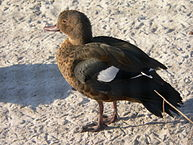
\includegraphics[width=4.3cm]{images/Ente}
    \caption{\small{Quelle: wikimedia}}
\end{wrapfigure}
Hier kommt nun viel Text. Hier kommt nun viel Text. Hier kommt nun viel Text. Hier kommt nun viel Text. Hier kommt nun viel Text. Hier kommt nun viel Text. Hier kommt nun viel Text. Hier kommt nun viel Text. Hier kommt nun viel Text. Hier kommt nun viel Text.  Hier kommt nun viel Text. Hier kommt nun viel Text. Hier kommt nun viel Text. Hier kommt nun viel Text. Hier kommt nun viel Text. Hier kommt nun viel Text. Hier kommt nun viel Text. Hier kommt nun viel Text. Hier kommt nun viel Text. Hier kommt nun viel Text. Hier kommt nun viel Text. Hier kommt nun viel Text. Hier kommt nun viel Text. Hier kommt nun viel Text. Hier kommt nun viel Text. Hier kommt nun viel Text. Hier kommt nun viel Text. Hier kommt nun viel Text. Hier kommt nun viel Text. Hier kommt nun viel Text. Hier kommt nun viel Text. Hier kommt nun viel Text. Hier kommt nun viel Text. Hier kommt nun viel Text. Hier kommt nun viel Text. Hier kommt nun viel Text. Hier kommt nun viel Text. Hier kommt nun viel Text. Hier kommt nun viel Text. Hier kommt nun viel Text.   Hier kommt nun viel Text.
\par\smallskip %Kleiner Absatz
Hier kommt nun viel Text. Hier kommt nun viel Text. Hier kommt nun viel Text. Hier kommt nun viel Text. Hier kommt nun viel Text. Hier kommt nun viel Text. Hier kommt nun viel Text. Hier kommt nun viel Text. Hier kommt nun viel Text. Hier kommt nun viel Text. Hier kommt nun viel Text. Hier kommt nun viel Text. Hier kommt nun viel Text.   Hier kommt nun viel Text. Hier kommt nun viel Text. Hier kommt nun viel Text. Hier kommt nun viel Text. Hier kommt nun viel Text. Hier kommt nun viel Text. Hier kommt nun viel Text. Hier kommt nun viel Text. Hier kommt nun viel Text. Hier kommt nun viel Text.   Hier kommt nun viel Text. Hier kommt nun viel Text. Hier kommt nun viel Text. Hier kommt nun viel Text. Hier kommt nun viel Text.   Hier kommt nun viel Text.
\par\bigskip %Großer Absatz

Damit die folgende Literaturliste angezeigt wird, müsst ihr eure Literatur in die bib.bib Datei eintragen und anschließend zunächst pdflatex ausführen, danach bibtex, danach wieder pdflatex.

\appendix
\section{Sample CSPs and Output}

\todo[inline]{Sample CSP mit Output}

\section{Commented Source Code}

\todo[inline]{Keine Ahnung ob wir das tun sollten... Vielleicht den entscheidenen Teil oder so?}

\bibliographystyle{plain}
\bibliography{bib}

\end{document}
